\documentclass{article}

\usepackage{Engineering}
\pdftitle{EFPLAB_1}

% === TEXT ===
\title{\textbf{Energies, fluids \& processes -- Laboratory \\ HSLU, Semester 2}}
\author{Matteo Frongillo}
\date{}

\begin{document}

\maketitle
\tableofcontents
\pagebreak

\section{Introduction to energies, fluids, and processes}
Energy exists in different forms and can neither be destroyed nor generated, but only
transformed.

\subsection{Energy forms}
\begin{minipage}{.45\textwidth}
    \begin{itemize}[itemsep=6pt]
        \item Potential energy: $E = mgh$
        \item Kinetic energy: $E = \frac{1}{2}mv^2$
        \item Thermal energy: $E = mc_p\Delta T$
        \item Light energy: $E = h\nu$
    \end{itemize}
\end{minipage}
\hfill
\begin{minipage}{.45\textwidth}
    \begin{itemize}[itemsep=6pt]
        \item Chemical energy: $E = mH$
        \item Electrical energy: $E = k\dfrac{q_1 q_2}{r}$
        \item Nuclear energy: $E = \Delta mc^2$
        \item Pressure energy (acoustic): $E = \dfrac{m p}{\rho}$
    \end{itemize}
\end{minipage}

\subsubsection{Important forms of energy for fluid motion}

\section{Fluids as energy carriers}
\subsection{Fluid definition}
\dots

\subsubsection{Properties of a fluid}
\pph{Density $\rho$}
Densitiy is a measure of working potential of a fluid:
\figbox{$\rho \triangleq \dfrac{m}{V}\ \left[\dfrac{kg}{m^3}\right]$}

where:
\begin{itemize}
    \item $m$ = mass;
    \item $V$ = volume.
\end{itemize}

\pph{Kinematic viscosity $\nu$}
Viscosity is a measure of the specific loss capacity of a fluid:
\figbox{$\nu \triangleq \dfrac{\mu}{\rho}\ \left[\dfrac{N\cdot s}{m^2} = Pa\cdot s\right]$}

where:
\begin{itemize}
    \item $\mu$ = dynamic viscosity
    \item $\rho$ = density
\end{itemize}

\begin{center}
    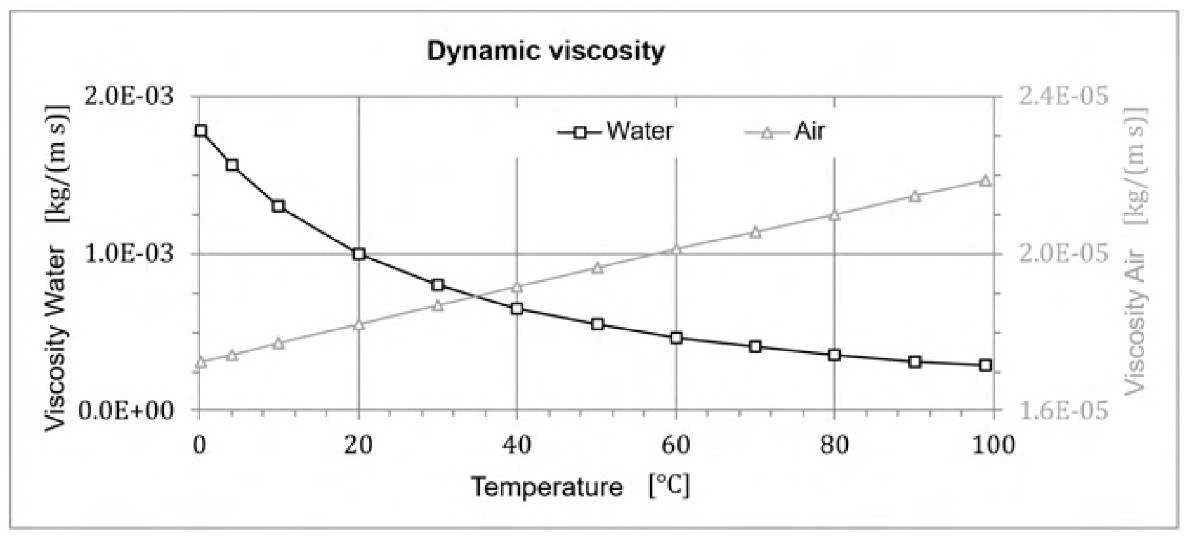
\includegraphics[width=.74\textwidth]{media/viscosity.png}
\end{center}

\rem{$\nu \propto \dfrac{1}{T}$}




\end{document}
